En préambule : 
\begin{pyverbatim}
import numpy as np
from math import exp, log
import matplotlib.pyplot as pl
\end{pyverbatim}

Il est utile de fixer en préambule les différentes constantes utilisées dans le TP.
\begin{pyverbatim}
T = [0, 7, 18, 27, 37, 56, 102]
C = [34.83, 32.14, 28.47, 25.74, 23.14, 18.54, 11.04]
\end{pyverbatim}

\question{}
\begin{pyverbatim}
def trace_fonction(xmin,xmax,f,nom_de_fichier,lab=""):
    """Trace la courbe de f sur [xmin,xmax]
    Enregistre dans nom_de_fichier"""
    pl.clf()
    les_x = np.linspace(xmin,xmax,1000)
    les_y = [f(t) for t in les_x]
    pl.plot(les_x,les_y,label=lab)
    if lab != '' :
        pl.legend()
    pl.savefig(nom_de_fichier)
    pl.clf()
\end{pyverbatim}



\question{}
\begin{pyverbatim}
def trace_ajustement(X,Y,f,nom_de_fichier,lab='Courbe d ajustement'):
    """Trace la courbe de f et les points (X,Y)
    Enregistre dans nom_de_fichier"""
    pl.clf()
    pl.plot(X,Y, 'rx',label='Mesures expérimentales')
    les_x = np.linspace(min(X),max(X),1000)
    les_y = [f(t) for t in les_x]
    pl.plot(les_x,les_y,label=lab)
    pl.xlabel('Temps (s)')
    pl.ylabel('Concentration (mol / L)')
    pl.title('Évolution de la concentration en fonction du temps')
    pl.legend()
    pl.savefig(nom_de_fichier)
    pl.clf()
\end{pyverbatim}

\question{}
\begin{pyverbatim}
def L1(k):
    """L1(k)"""
    S = 0
    for i in range(len(T)) :
        S = S + (C[i]-C[0]*exp(-k*T[i]))**2
    return S/7
\end{pyverbatim}

\question{}
On utilise
\begin{pyverbatim}
trace_fonction(0,0.12,L1,'fig_L1.png','$L^1$')
\end{pyverbatim}
La fonction $L^1$ est infiniment dérivable et semble bien avoir un minimum autour de $0,01$.

\begin{center}
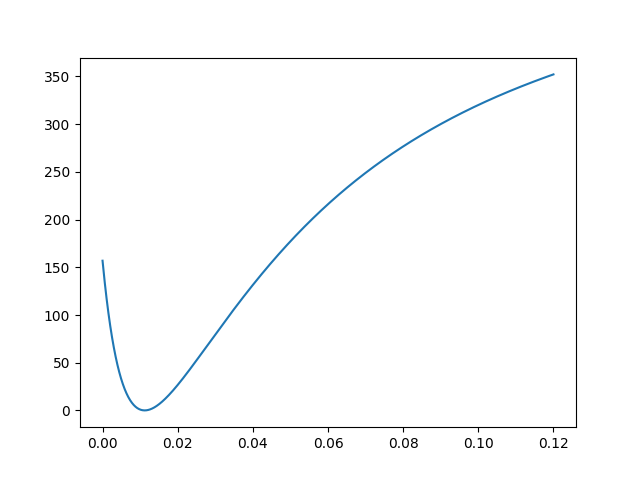
\includegraphics[width=0.5\textwidth]{tp12_durif_q4.png}
\end{center}


\question{}
C'est la dérivée de $L^1$ : 
\begin{equation*}
  dL^1 = (L^1)' : k \mapsto \dfrac{2C_0}{7} \sum_{i=0}^6 t_i (C_i-C_0\e^{-kt_i})\e^{-kt_i}.
\end{equation*}
\begin{pyverbatim}
def dL1(k):
    """L1'(k)"""
    S = 0
    for i in range(len(T)) :
        S = S + T[i] * (C[i]-C[0]*exp(-k*T[i])) * exp(-k*T[i])
    return 2*C[0]*S / 7
\end{pyverbatim}

\question{}
On dérive deux fois $L_1$.
\begin{equation*}
  (L^1)'' : k \mapsto \dfrac{2C_0}{7}\sum_{i=0}^6 t_i^2 (2C_0\e^{-kt_i}-C_i)\e^{-kt_i}.
\end{equation*}

\begin{pyverbatim}
def ddL1(k):
    """L1''(k)"""
    S = 0
    for i in range(len(T)) :
        S = S + T[i]**2 * (2*C[0]*exp(-k*T[i]) - C[i]) * exp(-k*T[i])
    return 2*C[0]*S / 7
\end{pyverbatim}

\question{}
\begin{pyverbatim}
def newton(f,fp,x0,eps):
    """Zéro de f par la méthode de Newton, critère d'arret eps
    fp : dérivée de f
    x0 : point initial"""
    u = x0
    v = u - f(u)/fp(u)
    while abs(v-u) > eps:
        u, v = v, v - f(v)/fp(v)
    return u
\end{pyverbatim}

\question{}
\begin{pyverbatim}
def val_k1() :
    """Valeur de k1"""
    return newton(dL1, ddL1, 0.01, 10**-10)

k1 = val_k1()
  
\end{pyverbatim}

\question{}
\begin{pyverbatim}
def f1(x) :
    """Fonction d'ajustement pour le modèle d'ordre 1"""
    return  C[0]*exp(-k1*x)

trace_ajustement(T,C,f1,'regression_ordre_1.png',"Ajustement pour le modèle d'ordre 1")
\end{pyverbatim}

\begin{center}
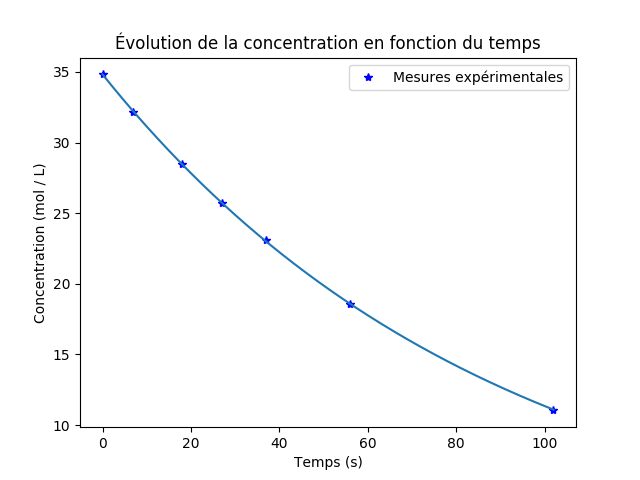
\includegraphics[width=0.5\textwidth]{tp12_durif_q9.png}
\end{center}

\question{}
\begin{pyverbatim}
def L2(k):
    """L2(k)"""
    S = 0
    for i in range(len(T)) :
        S = S + (C[i]-C[0]/(C[0]*k*T[i]+1))**2
    return S / 7   
\end{pyverbatim}

\question{}
La fonction $L^2$ est infiniment dérivable et semble bien avoir un minimum autour de $0,001$.
\begin{pyverbatim}
trace_fonction(0,0.05,L2,'fig_L2.png',"$L^2$")
\end{pyverbatim}

\begin{center}
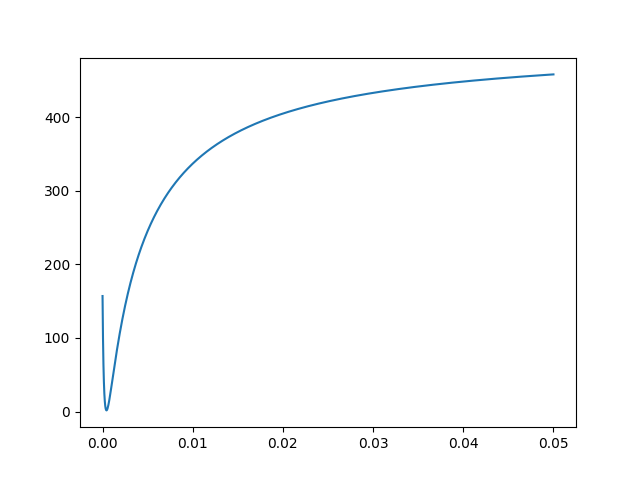
\includegraphics[width=0.5\textwidth]{tp12_durif_q11.png}
\end{center}

\question{}
C'est la dérivée de $L^2$ : 
\begin{equation*}
  dL^2 = (L^2)' : k \mapsto \dfrac{2C_0^2}{7} \sum_{i=0}^6 t_i \p{ \dfrac{C_i}{(1+C_0kt_i)^1} -\dfrac{C_0}{(1+C_0kt_i)^3}}.
\end{equation*}
\begin{pyverbatim}
def dL2(k):
    """L2'(k)"""
    S = 0
    for i in range(len(T)) :
        S = S + T[i] * (C[i]*C[0]*T[i]*k+C[i]-C[0]) / (C[0]*T[i]*k+1)**3
    return  2*S*C[0]**2 / 7 
\end{pyverbatim}

\begin{center}
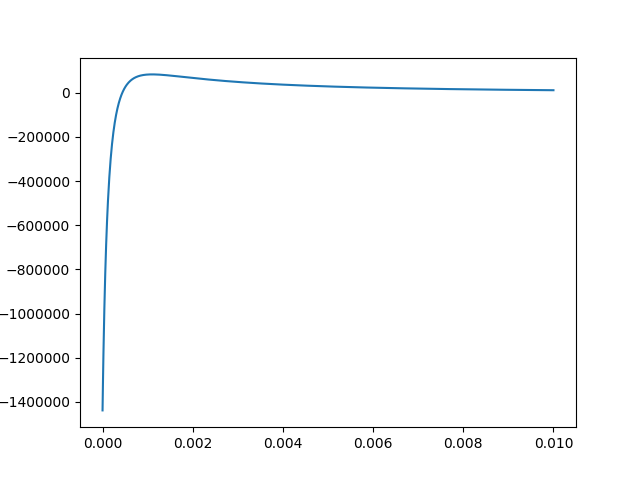
\includegraphics[width=0.5\textwidth]{tp12_durif_q12.png}
\end{center}


\question{}
\begin{pyverbatim}
def secante(f,x0,x1,eps):
    """Zéro de f par la méthode de la sécante"""
    u,v = x0,x1
    while abs(u-v) > eps : 
        p = (f(u)-f(v)) / (u-v)
        u,v = v,u - f(u)/p
    return u
\end{pyverbatim}

\question{}
\begin{pyverbatim}
def val_k2() :
    """Valeur de k2"""
    return secante(dL2,0.0005,0.0001,10**-10)
k2 = val_k2()  
\end{pyverbatim}

\question{}
\begin{pyverbatim}
def f2(x) :
    """Fonction d'ajustement pour le modèle d'ordre 2"""
    return  C[0]/(C[0]*k2*x+1)

trace_ajustement(T,C,f2,'regression_ordre_2.png',"Ajustement pour le modèle d'ordre 2")  
\end{pyverbatim}

\begin{center}
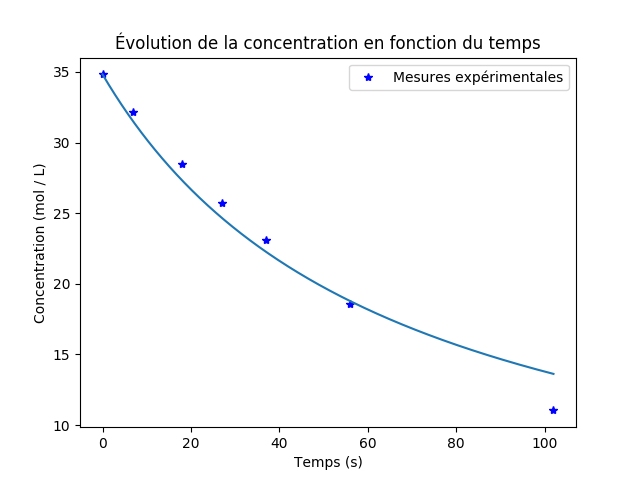
\includegraphics[width=0.5\textwidth]{tp12_durif_q15.png}
\end{center}

\question{}
\begin{pyverbatim}
def ddL2(k):
    """L2''(k)"""
    S = 0
    for i in range(len(T)) :
        S = S + T[i]**2 * (3*C[0]-2*C[i]-2*C[i]*C[0]*T[i]*k) / (C[0]*T[i]*k+1)**4
    return  2*C[0]**3 *S / 7

def val_k2_bis() :
    return newton(dL2, ddL2, 0.0001, 10**-10)
\end{pyverbatim}
La méthode de Newton est bien plus difficile à utiliser ici, si l'on se place un tout petit peu trop loin du minimum de $L^2$, alors elle ne converge pas.

\begin{center}
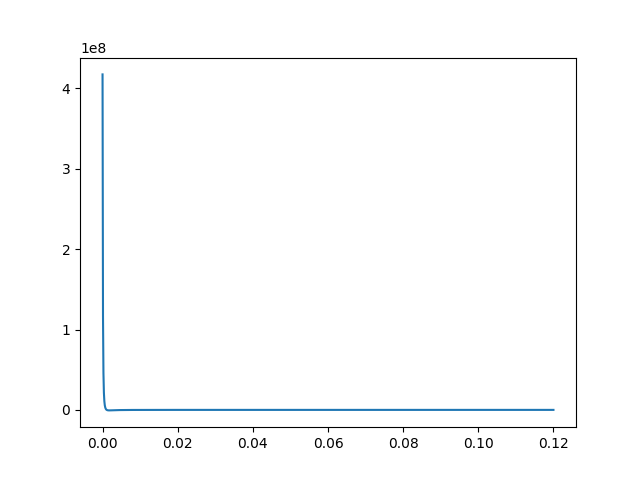
\includegraphics[width=0.5\textwidth]{tp12_durif_q16.png}
\end{center}


\question{}
Le second modèle est bien moins adapté que le premier aux données : la meilleure courbe solution coïncide bien moins aux données. De plus, la méthode de Newton y est plus difficile à appliquer (mais la celle de la sécante). 


\begin{center}
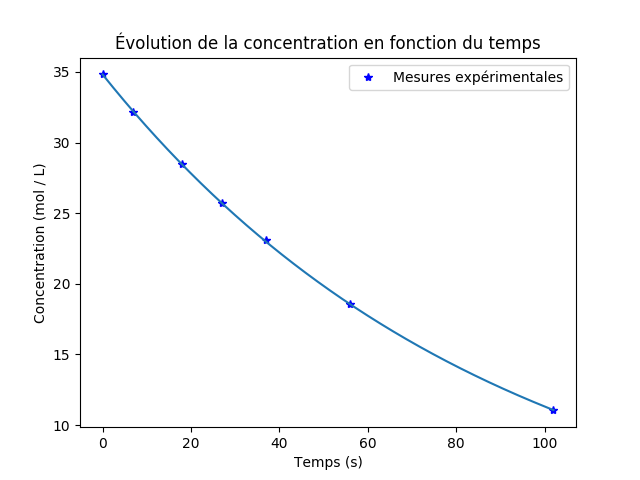
\includegraphics[width=0.5\textwidth]{tp12_durif_q17.png}
\end{center}


\question{}
C'est une simple fonction quadratique de coefficient dominant positif. Le minimum est atteint en 
\begin{equation*}
  -\dfrac{\sum_{i=0}^6 t_i \ln\p{\dfrac{C_i}{C_0}}}{\sum_{i=0}^6 t_i^2}.
\end{equation*}



\question{}
\begin{pyverbatim}
def val_kp1():
    """Valeur de k1'"""
    S1,S2 = 0,0
    for i in range(len(T)):
        S1 = S1 + T[i]*log(C[i]/C[0])
        S2 = S2 + T[i]**2
    return -S1/S2
    
kp1 = val_kp1()
\end{pyverbatim}

\question{}
\begin{pyverbatim}
def fp1(x) :
    """Fonction d'ajustement pour le modèle d'ordre 1
    Régression linéaire sur les logarithmes de C"""
    return  C[0]*exp(-kp1*x)


trace_ajustement(T,C,fp1,'regression_ordre_1_lin.png',"Modèle d'ordre 1, régression linéaire")
\end{pyverbatim}


\question{}
La méthode de Newton permet d'optimiser directement le critère souhaité, mais on n'obtient qu'un résultat approché. 
La méthode linéaire permet d'avoir une expression exacte (on dit aussi : forme close) du paramètre, mais le paramètre obtenu ne minimise pas le critère pertinent. 
Toutefois, le paramètre donné par la régression linéaire est très proche de celui donné par la méthode de Newton. 
